\section{Lebesgue Integration}

  Remember that Riemann integration is characterized by the approximation of step functions, which are the "building blocks" of Riemann integrable functions. To define the Lebesgue integral, we will start off with simple functions---which are a generalization of step functions. A function will be Lebesgue integrable if it can be approximated by these simple functions in some appropriate way. There are parallels between how we construct the Riemann and Lebesgue integral, namely that we can define the upper and lower integrals as the infimums and supremums of some set. However---while we were able to do this in ``one shot'' for the Riemann integral, the Lebesgue integral requires us to take intermediate steps. There are two ways that we can construct the Lebesgue integral. 
  \begin{enumerate}
    \item We define the integral for simple functions $\phi$ over finite measure. Since simple functions are made up of a linear combination of indicators, which are themselves bounded, the finite measure locks in the property that $\int \phi$ will be bounded. This allows us to take the integral of simple functions that have real-valued coefficients---both positive and negative---but is inherently limiting as we can't define the integral over infinite measures. With this, we can define the integral of bounded measurable functions using the lower and upper integrals. This is similar to the construction of the Riemann integral. Furthermore, if we want to define the general integral, we have to now restrict what we have built up into the nonnegative case---a bit unnatural. 

    \item We first define the integral for \textit{nonnegative} simple functions $\phi$ over any measure. We are sacrificing the ability to integrate negative simple functions early on, but this doesn't matter since we will split functions into a positive and negative part anyways. The true advantage of doing this is that we gain the ability to define integrals for infinite measures. This allows us to define for positive (possibly unbounded) measurable functions, and finally when we define the general Lebesgue integral, we deal with the $\infty - \infty$ problem by defining it only if at least one of the positive or negative integrals are finite. 
  \end{enumerate}

  I personally think the second way is superior, since in the end we can define integrals over infinite measure. Furthermore, since we are only working with positive functions, we only need to define the lower integral rather than checking to see if the lower and upper integrals coincide. 

  As we redefine these integrals over and over (sort of like method overriding), we really want to preserve three properties of the integral. 
  \begin{enumerate}
    \item Linearity. 
      \begin{equation}
        \int_E (\alpha f + \beta g) = \alpha \int_E f + \beta \int_E g 
      \end{equation}

    \item Monotonicity 
      \begin{equation}
        f \leq g \implies \int_E f \leq \int_E g 
      \end{equation}

    \item Additivity. 
      \begin{equation}
        A, B \text{ disjoint, measurable, and } E = A \cup B \implies \int_E f = \int_A f + \int_B f
      \end{equation}
  \end{enumerate}

\subsection{Simple Functions} 

  We will use $\phi, \varphi, \psi$ to denote simple functions. 

  \begin{definition}[Lebesgue Integral of Simple Functions over Finite Measure]
    Suppose $\phi = \sum_{k=1}^n a_k \chi_{E_k}: E \subset \mathbb{R} \to \mathbb{R}$ with $a_k \in \mathbb{R}$. 
    \begin{enumerate}
      \item If $m(E) < +\infty$, then we can define the integral which is guaranteed to be a finite number.  
      \begin{equation}
        \int_E \phi \coloneqq \sum_{k=1}^n a_k m(E_k)
      \end{equation} 

      \item If $a_k \geq 0$, we define the integral which lives in $\mathbb{R} \cup \{+\infty\}$.\footnote{As we have stated before, we could also define the Lebesgue integral of simple functions by letting $a_k$ takes values in $\mathbb{R}$. But then, we might have a case where $E = A \sqcup B$, with $m(A) = +\infty, m(B) = +\infty$, and $\phi = \chi_{A} - 2 \chi_{B} \implies \int_E \phi = \infty - \infty$. To prevent this from happening, some authors add the assumption that $m(E) < +\infty$, and I cover this case to make it as comprehensive as possible. }
      \begin{equation}
        \int_E \phi \coloneqq \sum_{k=1}^n a_k m(E_k)
      \end{equation} 
    \end{enumerate}
    This is well defined for any representation of $\phi$\footnote{We need this since the coefficients need not be unique. For example, we can write $1 \cdot \chi_{[0, 1]} + 1 \cdot \chi_{[0.5, 1]} = 1 \cdot \chi_{[0, 0.5]} + 2 \cdot \chi_{[0.5, 1]}$. If the $E_i$'s are disjoint, then this decomposition is unique and is called the \textbf{standard representation} of $\phi$. } 
  \end{definition} 
  \begin{proof}
    It is clear that the two definitions coincide if $m(E) < +\infty$ and $a_k \geq 0$ is true; it is the same formula.  
  \end{proof} 

  For bounded functions, we will temporarily focus on the first definition, and for general functions, we rely on the second definition. 

  \begin{theorem}[Properties of Lesbesgue Integral for Simple Functions]
    Suppose $\phi, \psi: E \subset \mathbb{R} \to \mathbb{R}$ are simple with $m(E) < +\infty$. Then, the following properties hold. 
    \begin{enumerate}
      \item Linearity. For $\alpha, \beta \in \mathbb{R}$, 
        \begin{equation}
          \int_E (\alpha \phi + \beta \psi) = \alpha \int_E \phi + \beta \int_E \psi
        \end{equation}

      \item Monotonicity. 
        \begin{equation}
          \phi \leq \psi \implies \int_E \phi \leq \int_E \psi 
        \end{equation}

      \item Additivity. If $A, B$ are disjoint, measurable, and $E = A \cup B$, then 
        \begin{equation}
          \int_E \phi = \int_A \phi + \int_B \phi
        \end{equation}
    \end{enumerate}
  \end{theorem}
  \begin{proof}
    Listed. 
    \begin{enumerate}
      \item We can subdivide sets s.t. $\phi$ and $\psi$ can be rewritten using the same finite family of sets $A_k$. 
      \item We can use (1) to rewrite 
        \begin{equation}
          \int_E \psi - \int_E \phi = \int \underbrace{(\psi - \phi)}_{\geq 0 \forall x} \geq 0
        \end{equation}

      \item Trivial by definition of simple functions. 
    \end{enumerate}
  \end{proof}

  \begin{example}[Step Function as Simple Function]
    For $a, b \in \mathbb{R}$, with $a < b$, let $f: [a, b] \longrightarrow \mathbb{R}$ be a step function. That is, there exists a partition $a = x_0 < x_1 < \ldots < x_n = b$ and constants $c_1, c_2, \ldots, c_n \in \mathbb{R}$ s.t. $f(x) = c_i$ for all $x \in (x_{i-1}, x_i)$ and each $i = 1, \ldots, n$. Then, $f$ is equal to the following simple function, taken over all open intervals and the points $x_j$ at the boundary of each interval. 
    \begin{equation}
      f = \sum_{i=1}^n c_i \chi_{(x_{i-1}, x_i)} + \sum_{j=0}^n f(x_j) \chi_{\{x_j\}}
    \end{equation}
    If we ignore the behavior of $f$ on the partition points $x_j$'s, then $f$ agrees almost everywhere with the simple function 
    \begin{equation}
      \sum_{i=1}^n c_i \chi_{(x_{i-1}, x_i)}
    \end{equation}
  \end{example} 

\subsection{Bounded Functions} 

  This isn't the most popular way to define Lebesgue integrability, but I'd like to compare it to Riemann integral. First, note that a Riemann integral 

  \begin{definition}[Lower, Upper Lebesgue Integral]
    Let $f: E \subset \mathbb{R} \to \mathbb{R}$ be bounded, with $m(E) < +\infty$. Then, the \textbf{upper and lower Lebesgue integrals} are defined 
    \begin{equation}
      \overline{L} f \coloneqq \inf_{\phi} \bigg\{ \int \phi \; \bigg| \; f \leq \phi, \phi \text{ simple} \bigg\}, \qquad \underline{L} f \coloneqq \sup_{\phi} \bigg\{ \int \phi \; \bigg| \; \phi \leq f, \phi \text{ simple} \bigg\}
    \end{equation}
    If the upper and lower Lebesgue integrals are equal, then $f$ is said to be \textbf{Lebesgue integrable}.
  \end{definition}

  This is exactly the same form as that of \hyperref[real-def:riemann-integral]{Riemann integration}. 

  \begin{definition}[]
    
  \end{definition}

\subsection{Positive Functions}

  If the $A_i$'s above are just intervals in $\mathbb{R}$, then $\phi$ reduces to a step function. But the entire problem with intervals is that they are too coarse. We can't work with them, so we generalize them to all measurable sets in $(X, \mathcal{A})$. The Riemann integral is built on an approximation scheme of a function, which we usually want to be continuous to satisfy this approximation, and so, if we want to build an approximation scheme for Lebesgue integrals, we want a similar scheme, i.e. if we take a sequence of simple measurable functions, I can get arbitrarily close to any measurable function $f$. This is exactly what we show below. 

  \begin{theorem}
    If $f: (X, \mathcal{A}) \longrightarrow [0, \infty]$ is measurable, there are simple measurable functions $f_k : (X, \mathcal{A}) \longrightarrow [0, \infty)$ s.t. 
    \begin{equation}
      f_k \leq f_{k+1} \text{ and } f = \lim_{k \rightarrow \infty} f_k
    \end{equation}
    where the inequalities and limits are pointwise. 
  \end{theorem}
  \begin{proof}
    We give a general picture of this proof for a function $f: \mathbb{R} \longrightarrow [0, \infty]$. We can first divide the codomain of the graph below into segments of $t = 1, 2, \ldots$, and take the preimage of all these units under $f$ to get $f_1$. More specifically, $A_1^t = f^{-1} ([t, \infty])$ for all $t$. By measurability of $f$, $A_1^t$ is measurable, and we can assign $f_1 = \chi_{A^1_1} + \chi_{A_1^2} \leq f$. 
    \begin{center}
        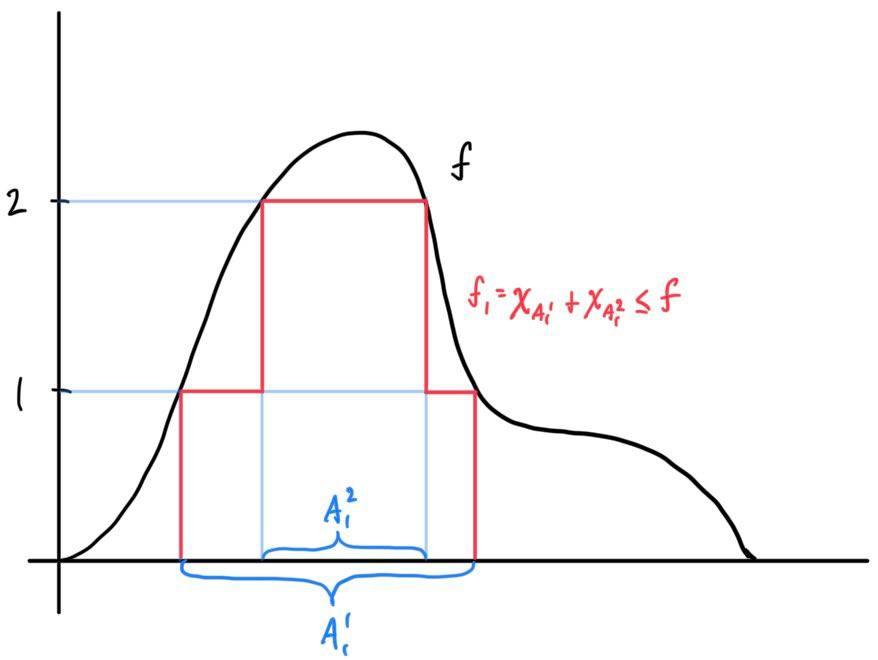
\includegraphics[scale=0.23]{img/Lebesgue_1.jpg}
    \end{center}
    Doing this again with finer subintervals of the codomain gives us, with $f_2 = \chi_{A_2^1} + \chi_{A_2^2} + \chi_{A_2^3} + \chi_{A_2^4} \leq f$. 
    \begin{center}
        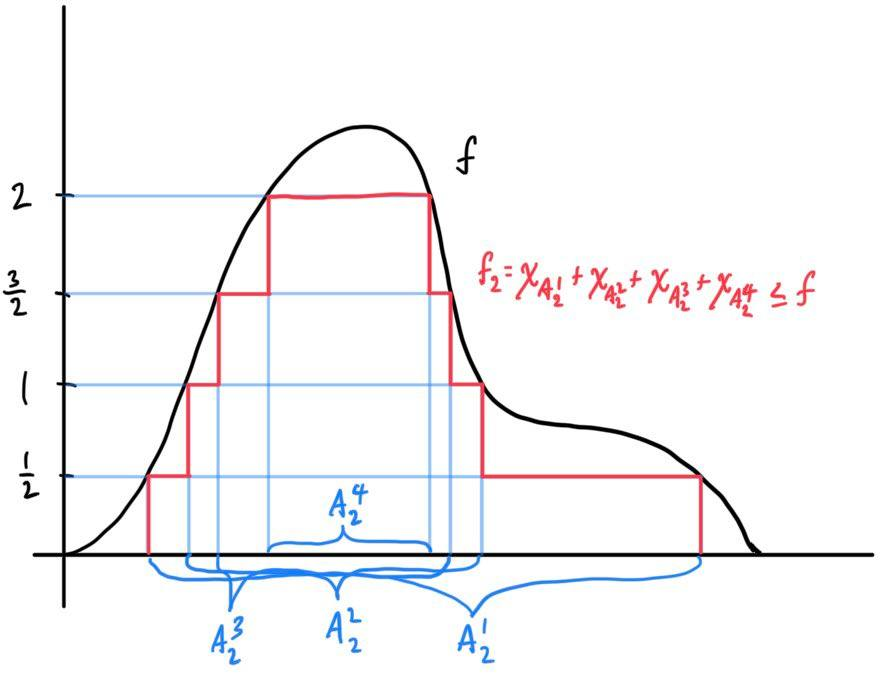
\includegraphics[scale=0.23]{img/Lebesgue_2.jpg}
    \end{center}
    and in general, we have $f_k = \sum_{j=1}^\infty \frac{1}{2^{k-1}} \chi_{A^j_k}$. But we said a simple function is a \textit{finite} sum, and if $\infty$ is in the range of $f$, then this becomes a problem. We can quickly fix this by just truncating the summation at a certain point in the codomain ($f_1$ only considers intervals up to $1$, $f_2$ up to $2$ and so on), ultimately giving us 
    \begin{equation}
      f_k = \sum_{j=1}^{k 2^{k-1}} \frac{1}{2^{k-1}} \chi_{A^j_k} 
    \end{equation}
  \end{proof}

  Finally, we can learn how to integrate. We require the positiveness condition on $f$ below because our previous theorem on approximating arbitrary functions with simple measurable functions $f_k$ requires that it be positive, too. 

  \begin{definition}[Lebesgue Integral of Positive Simple Functions]
    If $f = \sum_{k=1}^n c_k \chi_{A_k}$ is a positive simple Lebesgue measurable function on measure space $(X, \mathcal{A}, \mu)$, then the \textbf{Lebesgue integral} of $f$ is 
    \begin{equation}
      \int f \, d\mu = \sum_{k=1}^n c_k \mu(A_k)
    \end{equation}
  \end{definition}

  This Lebesgue integral agrees with the Riemann integral for step functions. Let $c_1, \ldots, c_n \in [0, \infty)$ and $a = x_0 < x_1 < \ldots < x_n = b$ be a partition. Let $f: [a, b] \longrightarrow [0, \infty]$ be a step function taking the value $c_i$ on the interval $(x_{i-1}, x_i)$ for $i = 1, \ldots, n$. Then the Riemann integral of $f$ is simply 
  \begin{equation}
    \int f(x) \,dx = \sum_{i=1}^n c_k |x_i - x_{i-1}|
  \end{equation}
  The Lebesgue integral is 
  \begin{align*}
    \int f \, d \mu & = \sum_{i=1}^n c_i \mu((x_{i-1}, x_i)) + \sum_{j=0}^n f(x_j) \mu(\{x_j\}) \\
    & = \sum_{i=1}^n c_k |x_i - x_{i-1}|
  \end{align*}
  which agrees with the Riemann integral. In the Riemann integral, we write $dx$ to indicate the variable that is being integrated over, but in the Lebesgue integral, we write $d \mu$, the measure which we are integrating over. Therefore, there are many possible values that can come out of a Lebesgue integral of a certain function, while a Riemann integral outputs only one value if exists. 

  \begin{example}
    Consider the simple function (consisting of one characteristic function) $\chi_{\mathbb{Q} \cap [0, 1]}$. $\mathbb{Q} \cap [0, 1]$ is a Lebesgue measurable set of $\mathbb{R}$, and we have $\chi_{\mathbb{Q} \cap [0, 1]} \geq 0$, so its Lebesgue integral is given by the above definition: 
    \begin{equation}
      \int_{\mathbb{R}} \chi_{\mathbb{Q} \cap [0, 1]} \, d\lambda = 1 \cdot \lambda(\mathbb{Q} \cap [0, 1]) = 0
    \end{equation}
  \end{example} 

\subsection{Positive Measurable Functions}

  \begin{definition}[Lebesgue Integral on Positive Measurable Functions]
    If $f: (X, \mathcal{A}, \mu) \longrightarrow [0, \infty]$ is measurable, then 
    \begin{equation}
      \int_X f \, d\mu = \sup \Big\{ \int g\, d\mu \,\Big|\, g \text{ simple }, g \leq f\Big\}
    \end{equation}
  \end{definition}

  Unlike Riemann integration, which looks at both the supremum and infimum of integrals of simple functions, Lebesgue integration only looks at the supremum, given that $f$ is nonnegative, so for all these $f$, the Lebesgue integral always exists. Defining Lebesgue integration for all real-valued functions, requires a simple extension. 

  \begin{definition}[Lebesgue Integral]
    Given a function $f: (X, \mathcal{A}, \mu) \longrightarrow \mathbb{R}$, we can split $f$ into a positive and negative part: 
    \begin{equation}
      f = f^+ - f^-
    \end{equation}
    where $f^+ = \max(f, 0)$ and $f^- = \max(-f, 0)$. Then, the Lebesgue integral of $f$ is 
    \begin{equation}
      \int f \, d \mu = \int f^+ \, d\mu - \int f^- \, d\mu
    \end{equation}
    given that at least one of these integrals is finite. If one is infinite and the other is finite, then we can call it infinite. If we have \textit{both} infinite integrals, then the integral doesn't exist. It has the properties: 
    \begin{enumerate}
      \item Monotonicity: 
      \begin{equation}
        g \leq f \implies \int g \, d\mu \leq \int f\, d\mu
      \end{equation}

      \item Scalar Multiplication: 
      \begin{equation}
        \int c f \, d\mu = c \int f \, d\mu
      \end{equation}

      \item Addition:
      \begin{equation}
        \int f + g \, d\mu = \int f \,d\mu + \int g \,d\mu
      \end{equation}
    \end{enumerate}
  \end{definition}

  Since $|f| = f^+ + f^-$, $f$ is also Lebesgue integrable if 
  \begin{equation}
    \int |f| \, d\mu < \infty 
  \end{equation}
  since by triangle inequality, we have 
  \begin{equation}
    \bigg| \int f \, d\mu \bigg| \leq \int |f| \, d \mu
  \end{equation}

  \begin{definition}
    The set of all functions $f: (X, \mathcal{A}, \mu) \longrightarrow \mathbb{R}$ that are Lebesgue integrable is denoted $\mathcal{L}^1(X, \mathcal{A}, \mu; \mathbb{R})$, or for short $\mathcal{L}^1(X, \mathcal{A}, \mu)$. 
  \end{definition}

  \begin{theorem}
    Suppose $f: (\mathbb{R}, \mathcal{A}, \mu) \longrightarrow \mathbb{R}$ is $0$ almost everywhere. Then $f$ is Lebesgue integrable with 
    \begin{equation}
      \int_\mathbb{R} f \, d\mu = 0 
    \end{equation}
    If $g: \mathbb{R} \longrightarrow \mathbb{R}$ is such that $f = g$ $\mu$-almost everywhere, then
    \begin{equation}
      \int_\mathbb{R} f\, d\mu = \int_\mathbb{R} g \, d\mu
    \end{equation}
  \end{theorem}

\subsection{Monotone Convergence Theorem}

  From now on, we will assume that all spaces $X$ are measure spaces $(X, \mathcal{A}, \mu)$ and all functions $f$ are measurable functions. The huge problem with Riemann integrals is that this theorem doesn't hold, but it is the case for Lebesgue integration. 

  \begin{theorem}[Monotone Convergene Theorem (MCT)]
    Given a nondecreasing sequence of measurable functions $f_1 \leq f_2 \leq f_3 \leq \ldots : X \longrightarrow [0, \infty]$, its limit $\lim_{k \rightarrow \infty} f_k$ always exists (since $f_k$ is nondecreasing), is measurable, and 
    \begin{equation}
      \int \lim_{k \rightarrow \infty} f_k \, d\mu = \lim_{k \rightarrow \infty} \int f_k \, d\mu
    \end{equation}
    This allows us to integrate the limit of nice functions $f_k$ by integrating these $f_k$ first and then finding what the values converge to. 
  \end{theorem}

\subsection{Riemann vs Lebesgue Integral}

  \begin{theorem}
    $f: \mathbb{R} \longrightarrow \mathbb{R}$ is Riemann integrable iff it is continuous $\lambda$ almost everywhere. If so, then $f$ is Lebesgue measurable and 
    \begin{equation}
      \int_{[a, b]} f \,d\lambda = \int_a^b f \, dx
    \end{equation}
    for all $a < b \in \mathbb{R}$. 
  \end{theorem}


